% LaTeX 2e Document.
% 
% $Id: sort.tex,v 1.4 2006/04/19 10:27:12 vdmtools Exp $
% 

%%%%%%%%%%%%%%%%%%%%%%%%%%%%%%%%%%%%%%%%
% PDF compatibility code. 
\makeatletter
\newif\ifpdflatex@
\ifx\pdftexversion\@undefined
\pdflatex@false
%\message{Not using pdf}
\else
\pdflatex@true
%\message{Using pdf}
\fi

\newcommand{\latexorpdf}[2]{
  \ifpdflatex@ #2
  \else #1
  \fi
}

\newcommand{\pformat}{a4paper}

\makeatother
%%%%%%%%%%%%%%%%%%%%%%%%%%%%%%%%%%%%%%%%

\latexorpdf{
\documentclass[\pformat,12pt]{jarticle}
}{
\documentclass[\pformat,pdftex,12pt]{jarticle}
}


\usepackage[dvips]{color}
\usepackage{longtable}
\usepackage{alltt}
\usepackage{graphics}
\usepackage{vpp}
\usepackage{makeidx}
\makeindex

\definecolor{covered}{rgb}{0,0,0}      %black
%\definecolor{not_covered}{gray}{0.5}   %gray for previewing
%\definecolor{not_covered}{gray}{0.6}   %gray for printing
\definecolor{not_covered}{rgb}{1,0,0}  %red

\newcommand{\InstVarDef}[1]{{\bf #1}}
\newcommand{\TypeDef}[1]{{\bf #1}}
\newcommand{\TypeOcc}[1]{{\it #1}}
\newcommand{\FuncDef}[1]{{\bf #1}}
\newcommand{\FuncOcc}[1]{#1}
\newcommand{\MethodDef}[1]{{\bf #1}}
\newcommand{\MethodOcc}[1]{#1}
\newcommand{\ClassDef}[1]{{\sf #1}}
\newcommand{\ClassOcc}[1]{#1}
\newcommand{\ModDef}[1]{{\sf #1}}
\newcommand{\ModOcc}[1]{#1}

%\newenvironment{vpp}
%{\noindent \rule{\columnwidth}{0.5pt} \begin{alltt}}
%{\end{alltt} \rule{\columnwidth}{0.5pt}}


\begin{document}
\vdmtoolsmanualscsk{VDM++ ソートアルゴリズム}{2.0}

\section{はじめに}

本書は、ソートの例題を1つ収めている。
クラス図は、図 \ref{inh}で見ることができる。
この例題の構造は、 \textit{strategy}パターンとして知られているものである。
このパターンはアルゴリズムの集団を定義するもので、それぞれ隠蔽し合い交換可能となっている。
\textit{strategy} パターンは、それを用いるクライアントから独立したものとしてアルゴリズムを変化させる。
異なるソートアルゴリズムを複数用いるクライアントとして、 \texttt{SortMachine} クラスが置かれている。
 \texttt{Sorter} クラスは、サポートされるアルゴリズムすべてに対して共通なインターフェイスを定義している抽象クラスである。


\begin{figure}[tbh]
\begin{center}
\mbox{}
\resizebox{12cm}{!}{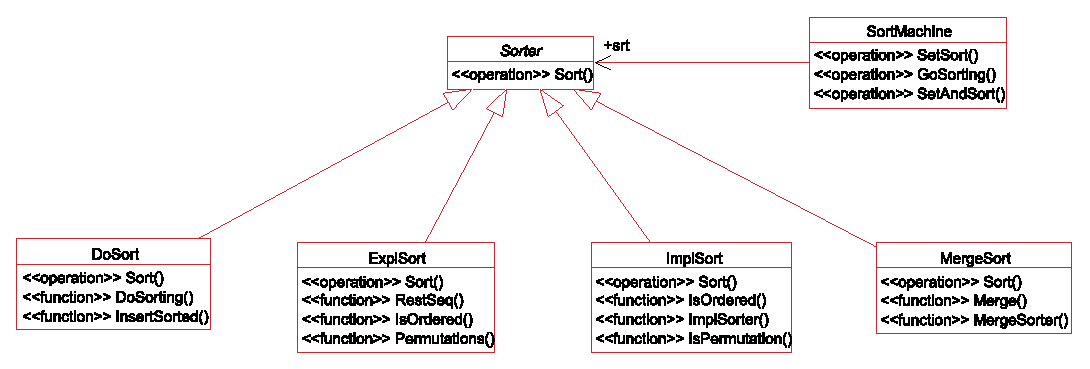
\includegraphics{inherit2}}
\caption{ソート例題のクラス図}\label{inh}
\end{center}
\end{figure}

\newpage
\input{sortmachine.vpp.tex}

\newpage
\input{sorter.vpp.tex}

\newpage
\input{mergesort.vpp.tex}

\newpage
\input{dosort.vpp.tex} % WHAT
%    The dosort algorithm. 
% ID
%    $Id: dosort_tc.tex,v 1.1 2006/04/07 04:38:18 vdmtools Exp $
% PROJECT
%    Toolbox
% COPYRIGHT
%    (C) 2012 SCSK

\begin{tabular}{p{25mm}l}
{\bf Test Suite :} & vdm.tc \\ 
{\bf Class :} & DoSort \\ 
\end{tabular}

\begin{longtable}{|l|r|r|}\hline
{\bf InsertSorted} & {\bf \#Calls} & {\bf Coverage} \kill
{\bf Name} & {\bf \#Calls} & {\bf Coverage} \\ \hline\hline
\endhead
DoSort`DoSorting & 6 & $\surd$ \\ \hline
DoSort`InsertSorted & 13 & $\surd$ \\ \hline
DoSort`Sort & 1 & $\surd$ \\ \hline
\hline
{\bf Total Coverage} & & {\bf 100\%} \\ \hline
\end{longtable}





\newpage
\input{implsort.vpp.tex}

\newpage
\input{explsort.vpp.tex}

%\include{sortmachine.vpp}
%
%\include{sorter.vpp}
%
%\include{mergesort.vpp}
%
%\include{dosort.vpp}
%
%\include{implsort.vpp}
%
%\include{explsort.vpp}

\newpage
\addcontentsline{toc}{section}{Index}
\printindex


\end{document}
